%An alternative ML approach was not performed in the \olep channel because of manpower limitations.
In the 1-lepton channel, an alternative ML approach (from here on called DNN) is trained in order to improve the sensitivity of the VBS signal in the analysis. The alternative approach utilizes neural networks (Keras models) which consist of a series of dense (fully-connected) layers. The ReLu (rectified linear unit) activation function is used for the hidden layers. The L2 regularization technique is used in order to surpress
overtraining. The sigmoid activation function used in the output yields a continuous output of the DNN scores.
More details of the neural network are summaried in Tab. \ref{tab:1lepDNN layers}.

\begin{table}[ht]
    \centering
    \begin{tabular}{c|c|c|c}
     Layer(type) & Number of Neurons & Activation Functions & Regularizers\\
     \hline
     \hline
     Layer1(dense) & 64 & ReLu & L2\\
     Layer2(dense) & 32 & ReLu & L2\\
     Layer3(dense) & 32 & ReLu & L2\\
     Layer4(dense) & 32 & ReLu & L2\\
     Layer5(dense) & 16 & ReLu & L2\\
     Layer Out(dense) & 1 & Sigmoid & -\\
    \end{tabular}
    \caption{1-lepton DNN strcture in merged and resolved signal regions.}
    \label{tab:1lepDNN layers}
\end{table}

The importance of input features for the trained neural networks is measured using the so-called SHAP (SHapley Additive exPlanation) values as proposed in the NeurIPS paper. 
%url = {https://proceedings.neurips.cc/paper/2017/file/8a20a8621978632d76c43dfd28b67767-Paper.pdf}
The goal of SHAP is to explain the model prediction for an event by estimating how much each input feature contributes to the final decision (DNN score).
For a complex model, like a neural network, its interpretalbe approximation can serve as a simpler explanation model. The simpler explanation model represents the original model and is easier to understand. 
Deep SHAP, a high-speed approximation algorithm, is the natural model-specific approximation method for the trained DNNs and is used to compute the SHAP values in them. 
One half of the samples from each signal region is used for the SHAP values calculation.

In order to condense the DNN models, input features are eliminated based on SHAP value ranking through backward feature elimination. After each round of elimination, the DNNs are re-trained and the remaining input features are ranked based on their SHAP values again. For the final discrimination, 15 input features remain for the merged region and 17 input features remain for the resolved region. The selected input features for the merged and resolved regimes are listed in Tab. \ref{tab:1lepNN}. The variables related to the entire system of signal jets, di-lepton and tagging jets are denoted as "full system". Further fine tuning of this list of input features through this process is possible, but the effectiveness of fine tuning can be minimal since no uncertainties have been taken into consideration.

\begin{table}[ht]
    \centering
    \begin{tabular}{r|c|c}
     feature & merged & resolved\\
     \hline
     \hline
     signal jet(s) mass & $m(J^\text{sig})$ & $m(jj^\text{sig})$\\
     signal jet transverse momentum & $ - $ & $p_\text{T}(j^\text{sig}_\text{lead})$ and  $p_\text{T}(j^\text{sig}_\text{sublead})$\\
     signal jet width & $ - $ & $W(j^\text{sig}_\text{lead})$ and  $W(j^\text{sig}_\text{sublead})$\\
     dijet(signal jet) transverse momentum & $ - $ & $p_\text{T}(jj^\text{sig})$\\
     number of tracks associated to the signal jet(s) & $N_\text{trk}(J^\text{sig})$ & -\\
     multiplicity of B-tagged jets & $N(j^\text{B-tagged})$ & -\\
     multiplicity of forward jets & $N(j^\text{forward})$ & -\\
     multiplicity of track jets & - & $N(j^\text{track})$\\
     diboson mass & $m(V^\text{had}V^\text{lep})$ & $ - $\\
     leading tagging jet mass & $m(j^\text{tag}_\text{lead})$ & $ - $\\
     full system mass & $ - $ & $m(V^\text{had}V^\text{lep}+jj^\text{tag})$\\
     tagging jet transverse momentum & $p_\text{T}(j^\text{tag}_\text{sublead})$ & $p_\text{T}(j^\text{tag}_\text{lead})$ and $p_\text{T}(j^\text{tag}_\text{sublead})$\\
     tagging jet width & $W(j^\text{tag}_\text{lead})$ and $W(j^\text{tag}_\text{sub})$  & $ - $\\
     boson centrality & $\xi(V)$ & $ - $\\
     pseudo-rapidity of tagging jets & - & $\eta(j^\text{tag}_\text{lead})$ and $ \eta(j^\text{tag}_\text{sublead})$\\
     pseudo-rapidity of lepton & - & $\eta(l)$\\
     lepton transverse momentum & $p_\text{T}(l)$ & -\\
     jets multiplicity & \multicolumn{2}{c}{$N(j)$}\\
     number of tracks associated to the tagging jets & \multicolumn{2}{c}{$N_\text{trk}(j^\text{tag}_\text{lead})$ and $N_\text{trk}(j^\text{tag}_\text{sublead})$}\\
     tagging jets mass & \multicolumn{2}{c}{$m(jj^\text{tag})$}\\
     tagging jet separation & \multicolumn{2}{c}{$\Delta\eta(j^\text{tag}_\text{lead},j^\text{tag}_\text{sublead})$}\\
     lepton charge & \multicolumn{2}{c}{$Q(l)$}\\
    \end{tabular}
    \caption{Input variables for the 1-lepton DNN in merged and resolved signal regions.}
    \label{tab:1lepNN}
\end{table}

Separate models are trained in the two regimes.
For the merged regime, samples from the high purity and low purity signal regions are trained together in one model.
For the resolved regime, a separate model was trained in the resolved signal region.
In each regime the samples were split in half according to event number. One half is used for training the DNN and the other half is used for validation. Signal EW $VV+jj$ events are labelled as $"1"$ and background events are labelled as $"0"$.
Binary cross-entropy was chosen as the loss function.
The Adam and SGD (stochastic gradient descent) optimizers have been tested with the DNN models. The SGD optimizer is selected since its effect on a smoother distribution of the DNN scores. Fig. \ref{fig:1lepDNNoutputs} shows the DNN scores for all three signal regions. 

\begin{figure}[ht]
 \begin{center}
  \subfigure[DNN HP]{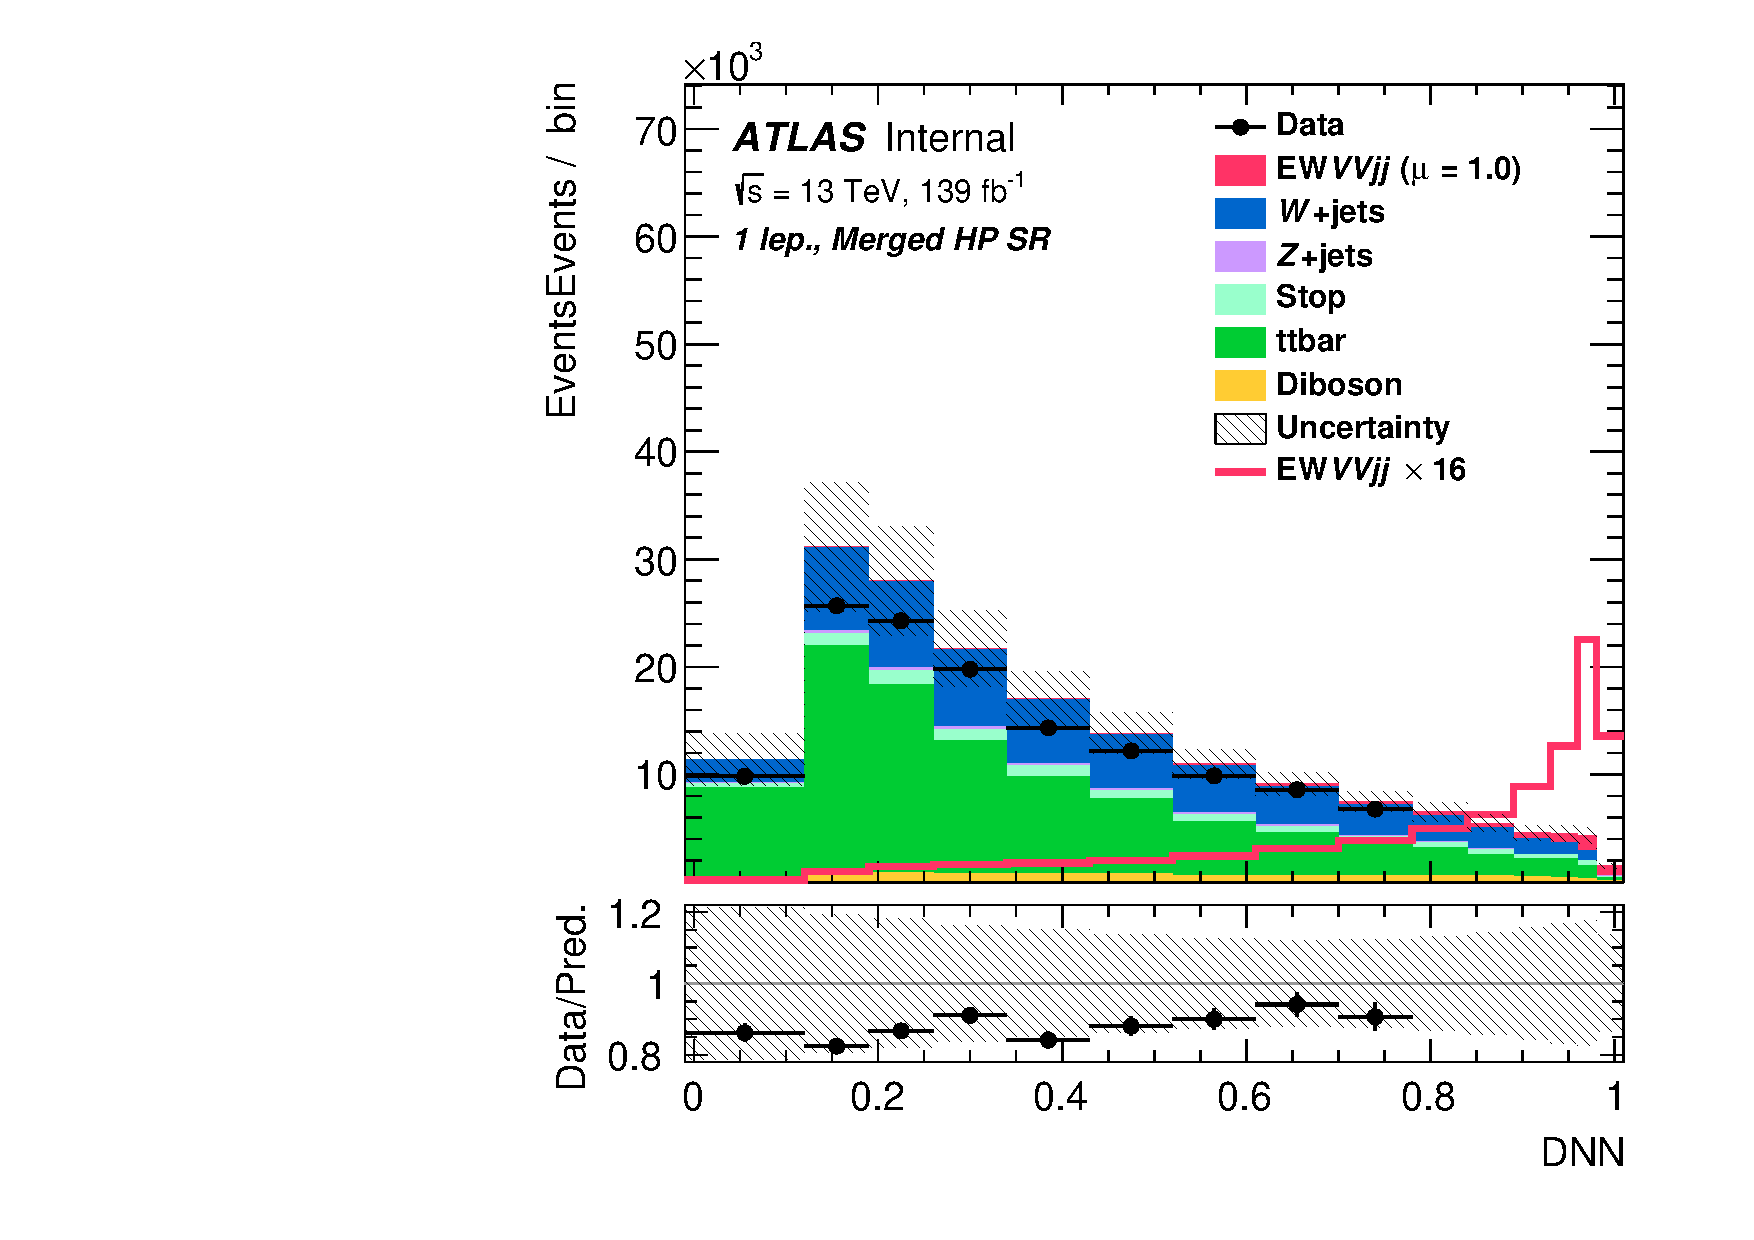
\includegraphics[width=0.3\textwidth]{figures/1lep/altML/Region_distDNN_DSRVBSHP_BMin0_J0_incJet1_L1_T0_incFat1_Y6051_incTag1_Fat1_Prefit.pdf}}
  \subfigure[DNN LP]{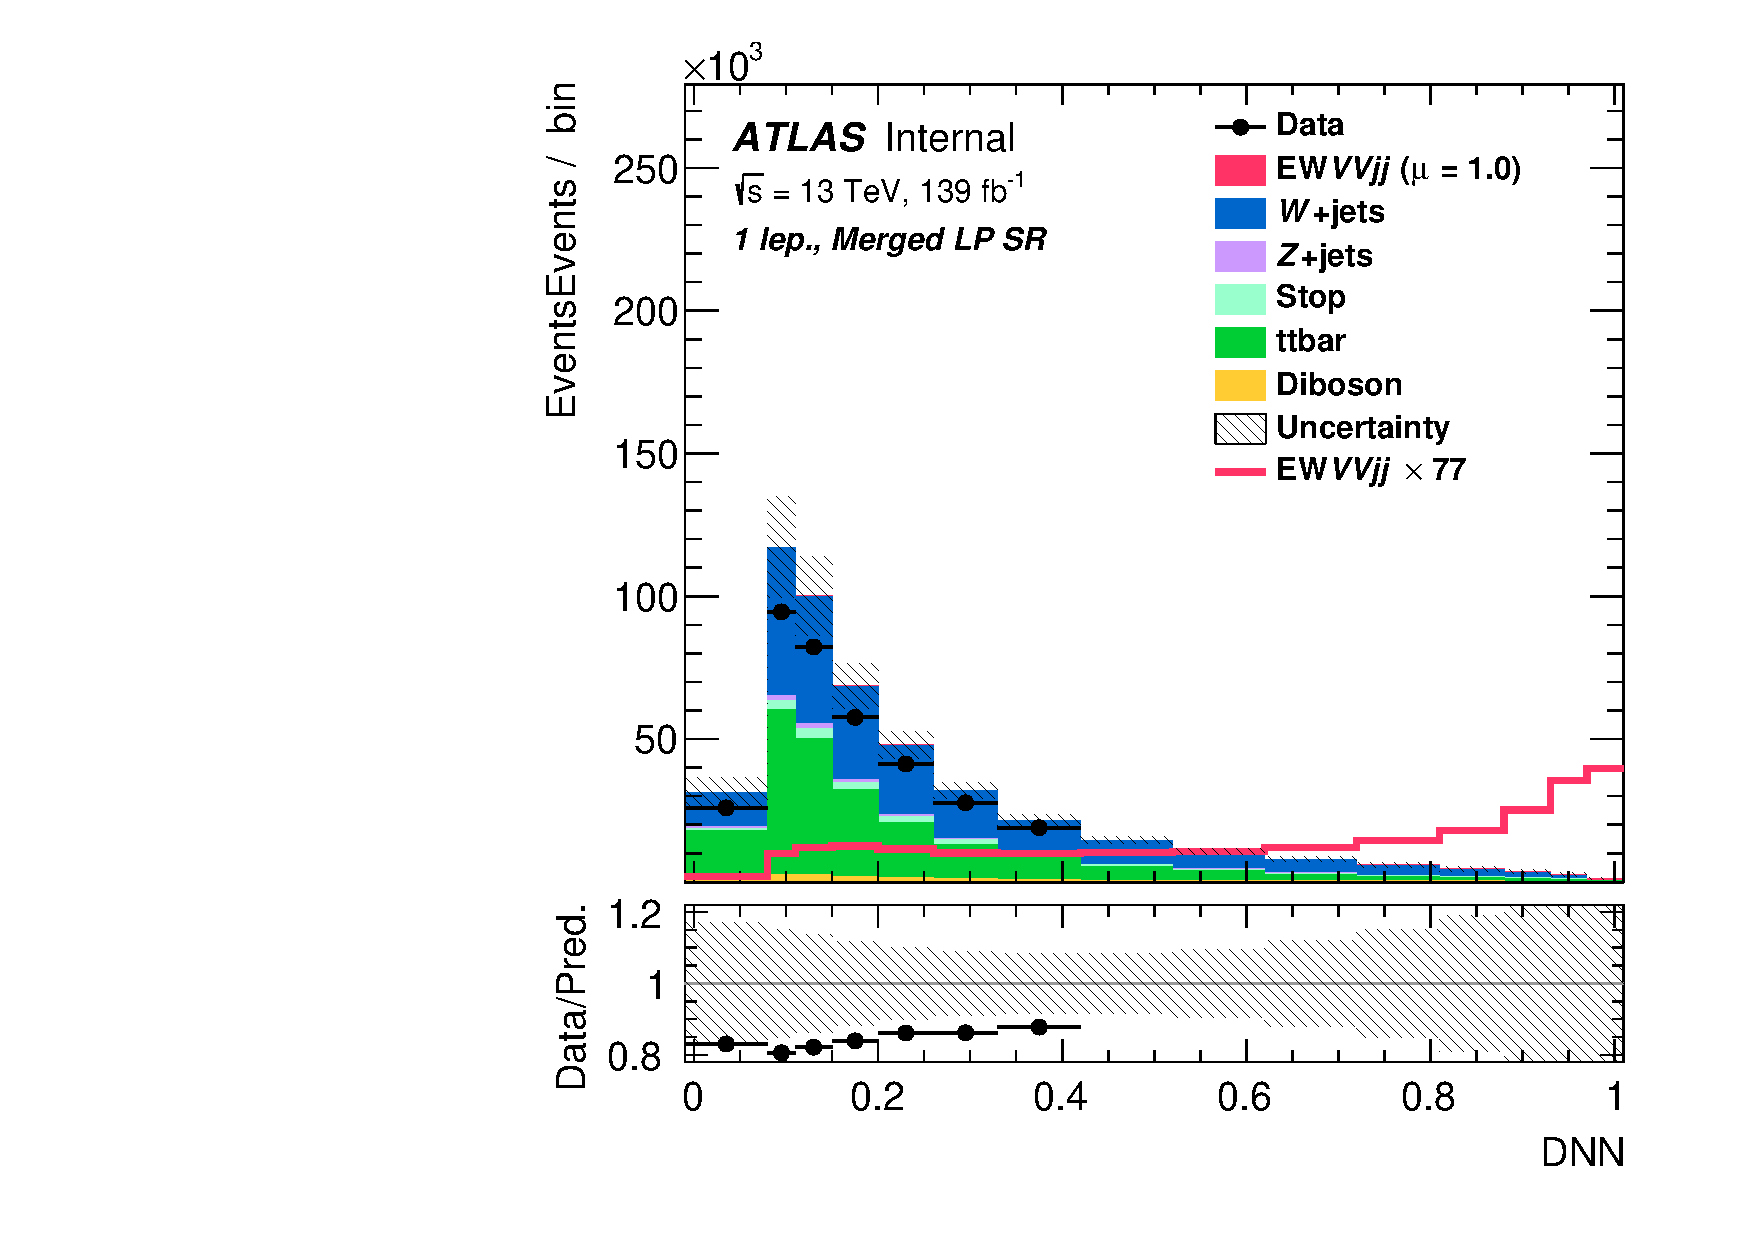
\includegraphics[width=0.3\textwidth]{figures/1lep/altML/Region_distDNN_DSRVBSLP_BMin0_J0_incJet1_L1_T0_incFat1_Y6051_incTag1_Fat1_Prefit.pdf}}
  \subfigure[DNN Res]{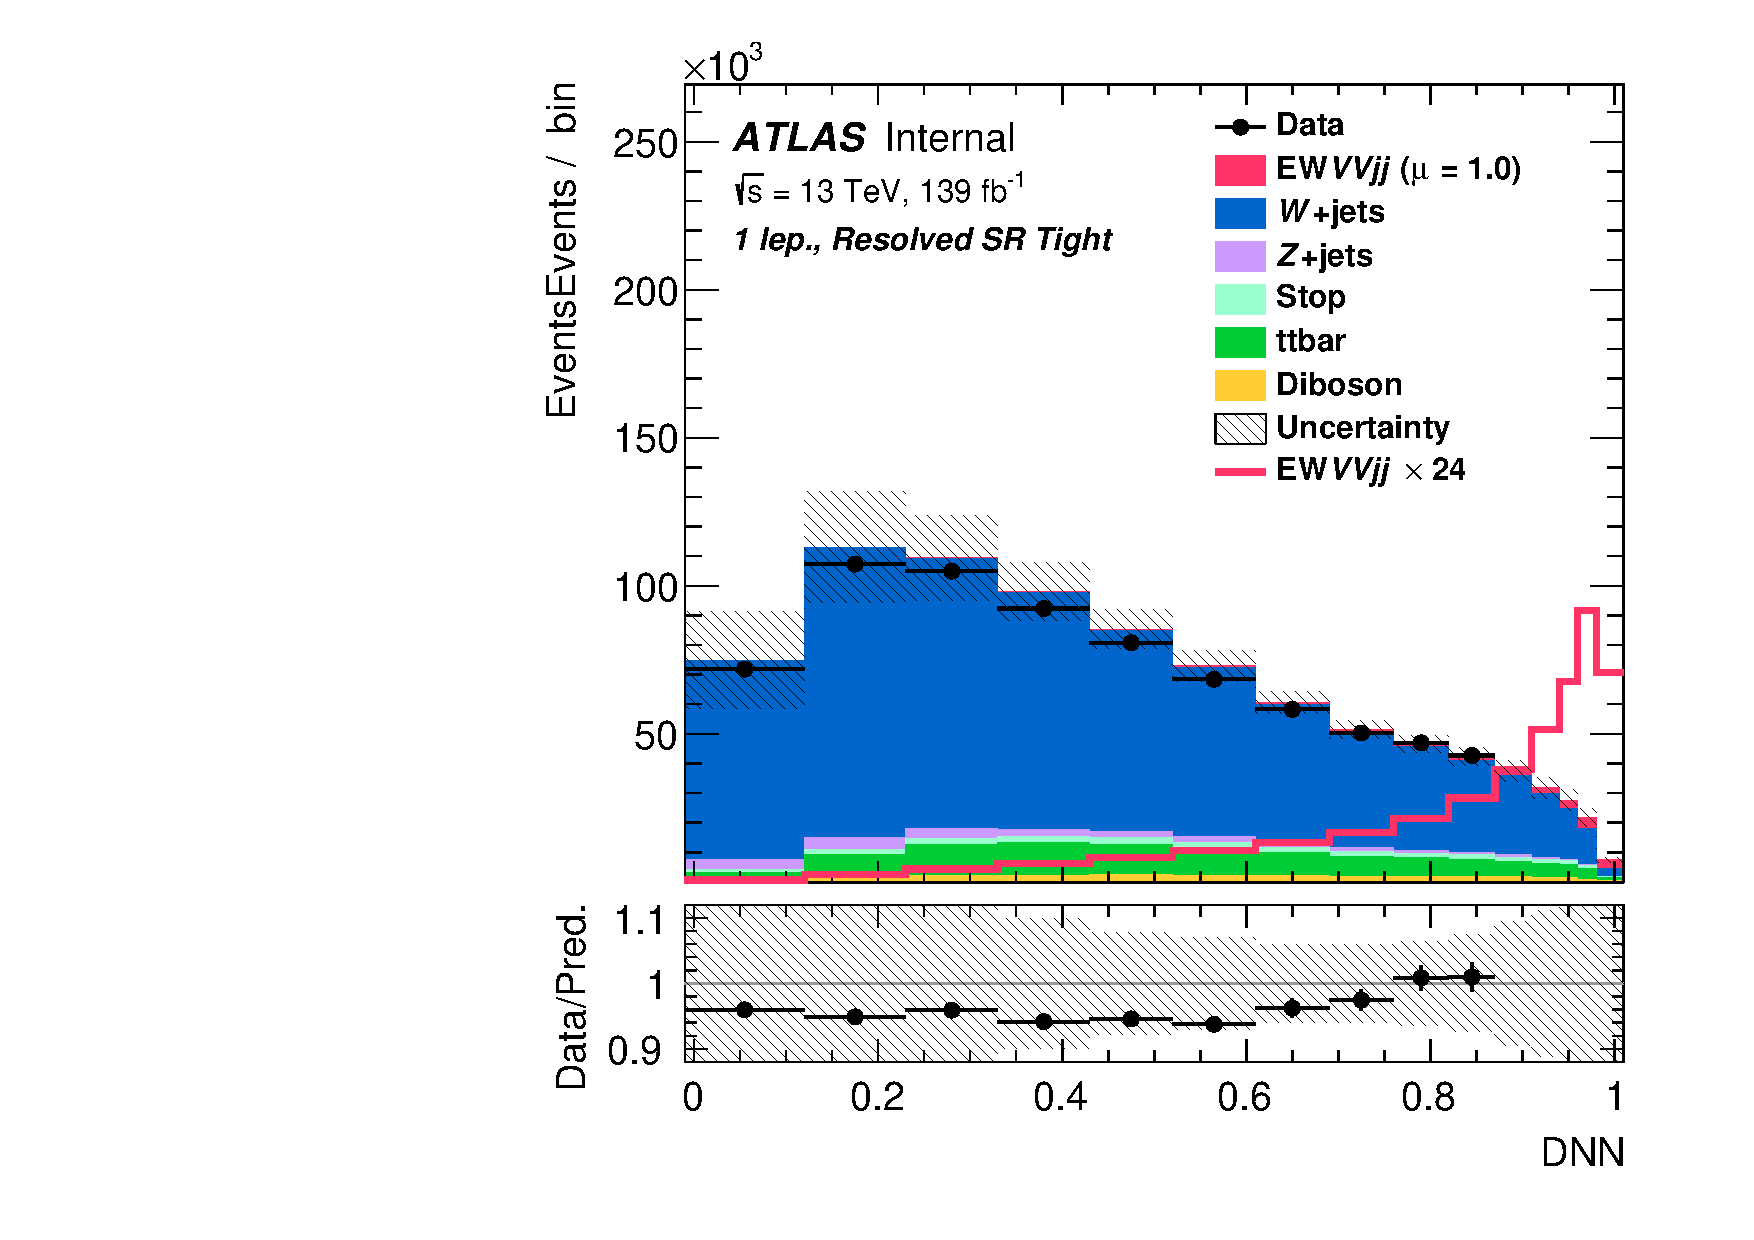
\includegraphics[width=0.3\textwidth]{figures/1lep/altML/Region_distDNN_DSRVBSTight_BMin0_T0_Y6051_incTag1_J2_L1_incJet1_Prefit.pdf}}
  \caption{Features of the NN MVA in the merged HP signal region.}
 \label{fig:1lepDNNoutputs}
 \end{center}
\end{figure}

%%\begin{figure}[ht]
%% \begin{center}
%%  \subfigure[tagging jet mass]{\includegraphics[width=0.3\textwidth]{figures/0lep/mvainputs/merged/plots/soverb_MTagJets_SRVBS_HP.pdf}}
%%  \subfigure[tagging jet $p_\text{T}$]{\includegraphics[width=0.3\textwidth]{figures/0lep/mvainputs/merged/plots/soverb_PtTagJet1_SRVBS_HP.pdf}}
%%  \subfigure[tagging jet $p_\text{T}$]{\includegraphics[width=0.3\textwidth]{figures/0lep/mvainputs/merged/plots/soverb_PtTagJet2_SRVBS_HP.pdf}}
%%  \subfigure[signal jet mass]{\includegraphics[width=0.3\textwidth]{figures/0lep/mvainputs/merged/plots/soverb_MFatJet_SRVBS_HP.pdf}}
%%  \subfigure[signal jet $p_\text{T}$]{\includegraphics[width=0.3\textwidth]{figures/0lep/mvainputs/merged/plots/soverb_PtFatJet_SRVBS_HP.pdf}}
%%  \subfigure[$E_\text{T}^\text{miss}$]{\includegraphics[width=0.3\textwidth]{figures/0lep/mvainputs/merged/plots/soverb_MET_SRVBS_HP.pdf}}
%%  \subfigure[signal jet-$E_\text{T}^\text{miss}$ separation]{\includegraphics[width=0.3\textwidth]{figures/0lep/mvainputs/merged/plots/soverb_DeltaPhiFatJet_MET_SRVBS_HP.pdf}}
%%  \subfigure[tracks assoc. to tagging jet]{\includegraphics[width=0.3\textwidth]{figures/0lep/mvainputs/merged/plots/soverb_NumTrkPt500TagJet1_SRVBS_HP.pdf}}
%%  \subfigure[tracks assoc. to tagging jet]{\includegraphics[width=0.3\textwidth]{figures/0lep/mvainputs/merged/plots/soverb_NumTrkPt500TagJet2_SRVBS_HP.pdf}}
%%  \caption{Features of the NN MVA in the merged HP signal region.}
%% \label{fig:0lepNNInputsMergedHP}
%% \end{center}
%%\end{figure}







